\begin{frame}
    \frametitle{Generator grafów}

    \begin{enumerate}
        \item Podstawa to biblioteka igraph
        \item Funkcyjna i modularna budowa
        \item Rysunki grafów
            \begin{enumerate}
                \item Rozmiar 800x600 pikseli
                \item Białe tło
                \item Pomarańczowe i nieoznaczone wierzchołki
                \item Zapisane w odpowiednich katalogach, odpowiadających klasie grafu
            \end{enumerate}
        \item Funkcje
            \begin{enumerate}
                \item Typ grafu - ścieżka, cykl, graf pełny, graf bezkrawędziowy, drzewo binarne
                \item Liczba grafów do wygenerowania
                \item Liczba wierchołków grafów
                \item Współczynnik odpowiadający~za zakrzywienie krawędzi
            \end{enumerate}
    \end{enumerate}

\end{frame}

\begin{frame}
    \frametitle{Generator grafów}

    \begin{figure}[ht]
        \centering
        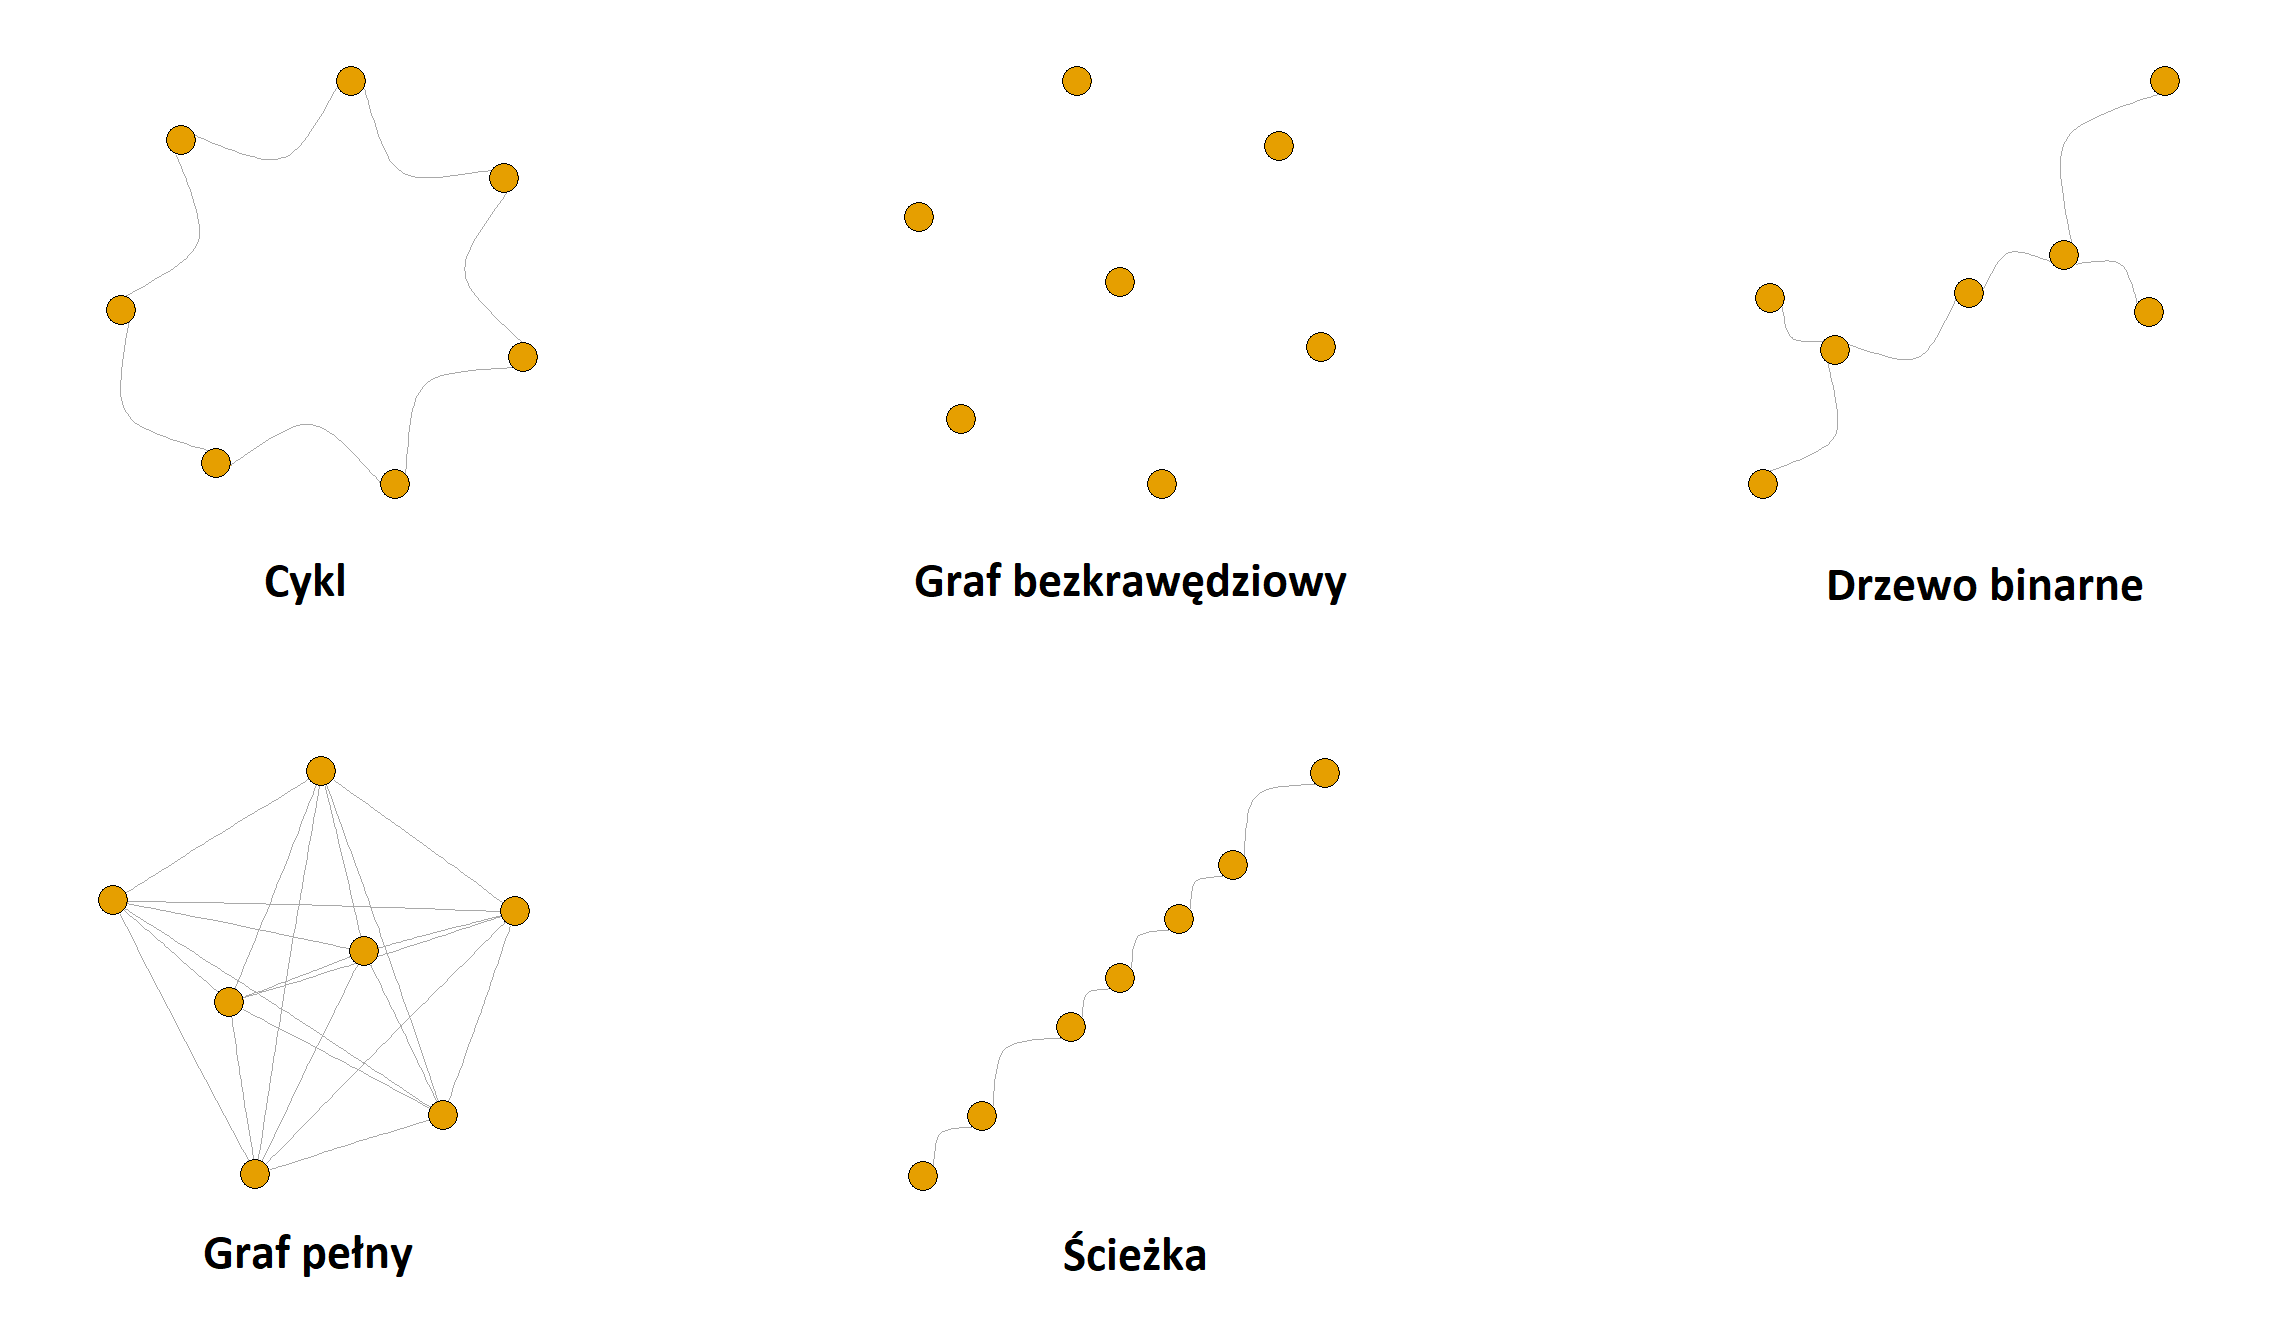
\includegraphics[height=6cm]{../thesis/resources/model/images/gen-graphs-generated.png}
        \caption{Przykładowe wygenerowane rysunki grafów z~każdej klasy}
    \end{figure}

\end{frame}